% Inhaltsverzeichnis
\newcommand{\mbtableofcontents}{
	\clearpage
	\lhead[ \leftmark   ]{\textbf{Inhaltsverzeichnis}}
	\tableofcontents
}

% Kapitel
\newcommand{\mbchapter}[1]{
	\chapter{#1}
	\lhead[ \leftmark   ]{\textbf{#1}}
}

% Abbildungsverzeichnis
\newcommand{\mblistoffigures}{
	\listoffigures
	\lhead[ \leftmark   ]{\textbf{Abbildungsverzeichnis}}}

% Tabellenverzeichnis
\newcommand{\mblistoftables}{
	\listoftables
	\lhead[ \leftmark   ]{\textbf{Tabellenverzeichnis}}
}

% Glossar
\newcommand{\mbprintglossaries}{
	\mbchapter{Glossar}
	\printglossary[title=,type=main]
}	

\newcommand{\mbprintabbreviation}{
	\mbchapter{Acronyms}
	\printglossary[title=,type=\acronymtype]
}	


% Literatur
\newcommand{\mbbibliography}{
	\mbchapter{Literaturverzeichnis}
	\printbibliography[title=, heading=none]
	\lhead[ \leftmark   ]{\textbf{Literaturverzeichnis}}
}

% Empty page
\newcommand{\mbemptypage}{
	\mbox{}
	\thispagestyle{empty}
	\newpage
}

% Beispiele

% Abbildungen	
%\begin{figure}
%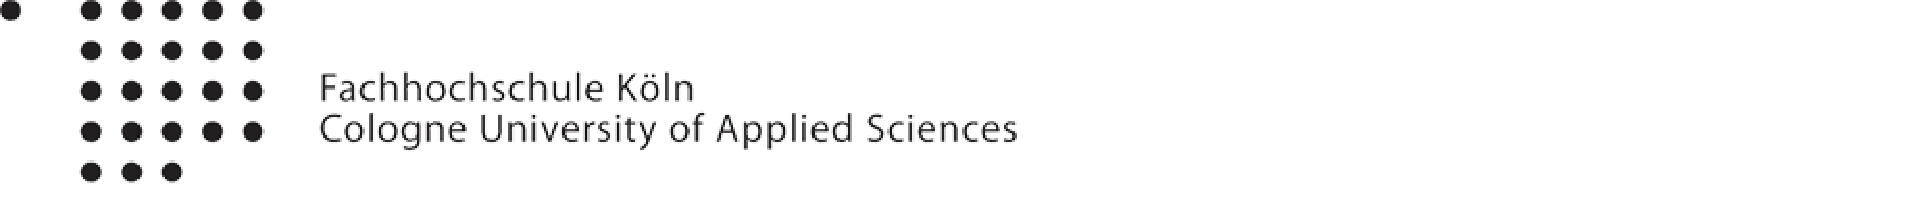
\includegraphics{Bilder/FHGummersbachLogo.pdf}
%\caption{Test}
%\end{figure}